\documentclass{beamer}

\usepackage{mytheme}

% For Title Page
% ---------------------------------------------------------------------------------------

\title{Applications of Galois Theory}

\author[Sandesh Thakuri]{Mr. Sandesh Thakuri}

\institute[CDM, TU]
{Central Department of Mathematics, TU}

\date{2080-12-24}


% Begin Document
% ---------------------------------------------------------------------------------------------------------------------

\begin{document}
\myfootline

\begin{frame}[plain]
  \tikzonlytitlepage
  \titlepage
\end{frame}

\begin{frame}[plain]
  \begin{tcolorbox}[colframe=blue!80!violet, boxsep=2mm,  title={\large \bfseries Outlines}]
    \tableofcontents
  \end{tcolorbox}
\end{frame}

% -----------------------------------------------------------------------------------------------------------------------
\small
\section{Galois Theory}
\subsection{Background}
\begin{frame}{Background}

  {\footnotesize  Let \(F\) be a field extension of a field \(K\).}
  \vspace{2mm}

  \begin{tcolorbox}[colframe=blue!40, boxsep=-1pt]
    \begin{definition}[K-automorphism]
      A field-automorphism \(\sigma \in Aut F\) which is also K-homomorphism is called K-automorphism. In other words, a field-automorphism \(\sigma \in Aut F\) that fixes K element-wise is called K-automorphism \cite{hunger}.
    \end{definition}
    \vspace{1mm}
    \begin{definition}[Galois Group]
      The group of all K-automorphisms of \(F\) is called the Galois group of \(F\) over \(K\) and it is denoted by \(Aut_K^F\) \cite{hunger}.
    \end{definition}
    \vspace{1mm}
    \begin{definition}[Galois Extension]
      Let \(F\) be an extension field of \(K\) such that the fixed field of the Galois group \(Aut_K^F\) is \(K\) itself. Then \(F\) is said to be a Galois extension of \(K\) or Galois over \( K\) \cite{hunger}.
    \end{definition}
  \end{tcolorbox}
\end{frame}

\begin{frame}{Fixed Field}
  Let \(E\) be an intermediate field and \(H\) be a subgroup of \(Aut_K^F\), then:
\begin{enumerate}
\item[i)] \(H' = \{v \in F \; | \: \sigma(v)=v,\) for all \(\sigma \in H \}\) is an intermediate field of the extension field \(F\) of \(K\);
\item[ii)] \(E' = \{\sigma \in Aut_K^F \; | \; \sigma(u)=u,\) for all \(u \in E\}=Aut_E^F\) is a subgroup of \(Aut_K^F\).
\end{enumerate}

The field \(H'\) is called the fixed field of the subgroup H in F \cite{hunger}.
\end{frame}

\subsection{Galois Correspondence}
\begin{frame}{Galois Correspondence}
    \begin{tcolorbox}[colframe=blue!40, boxsep=2mm]
  \begin{theorem}[Fundamental Theorem of Galois Theory]
  If \(F\) is a finite dimensional Galois extension of \(K\), then there is a one-to-one correspondence between the set of all intermediate fields of \(F\) over \(K\) and the set of subgroups of the Galois group \(Aut_K^F\) such that:
  \begin{enumerate}
  \item[i)] the relative dimension of two intermediate fields is equal to the relative index of the corresponding subgroups. In particular \(Aut_K^F\) has order \([F:K]\);
  \item[ii)] \(F\) is Galois over every intermediate field \(E\), but \(E\) is Galois over \(K\) if and only if the corresponding subgroup \(E'= Aut_E^F\) is normal in \(G=Aut_K^F\).In this case \(G/E'\) is isomorphic to the Galois group \(Aut_K^E\) of \(E\) over \(K\) \cite{hunger}.
  \end{enumerate}
\end{theorem}
\end{tcolorbox}
\end{frame}

\begin{frame}{Illustration of The Fundamental Theorem}
  \begin{minipage}{0.65\textwidth}
  Let \(F\) be an Galois extension of a field \(K\). Let the towers of the intermediate fields of \(F\) over \(K\) be as follows:
  \[
    K \subset E \subset F
  \]
\noindent
  Let \(G\) be the Galois group of \(F\) over \(K\). Then its subsets are
  \[
    \{e\} \subset H \subset G
  \]
  Then the one-to-one correspondence is as shown:
\end{minipage}
\begin{minipage}{0.3\textwidth}

  \begin{tcolorbox}[colback=orange!20, colframe=orange!80!black, title={\footnotesize \textcolor{white}{Galois-correspondence}}, width=4cm]
    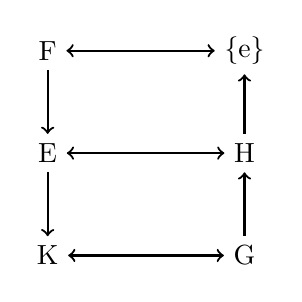
\begin{tikzpicture}
      \node (f) {F};
      \node[below of=f, yshift=-3mm] (e) {E};
      \node[below of=e, yshift=-3mm] (k) {K};

      \draw[->,thick] (f)--(e);
      \draw[->,thick] (e)--(k);

      \node[right of=f, xshift=15mm] (i) {\{e\}};
      \node[below of=i, yshift=-3mm] (h) {H};
      \node[below of=h, yshift=-3mm] (g) {G};

      \draw[<-, thick] (i)--(h);
      \draw[<-, thick] (h)--(g);

      \draw[<->, thick] (f)--(i);
      \draw[<->, thick] (e)--(h);
      \draw[<->, thick] (k)--(g);
    \end{tikzpicture}
  \end{tcolorbox}
\end{minipage}

\vspace{5mm}

 \begin{tcolorbox}[colframe=blue!40]
\begin{definition}[Remark]
  The intermediate fields are getting larger as we go from top to bottom  as the fields are getting extended. But the subgroups are getting smaller.
\end{definition}
\end{tcolorbox}
\end{frame}

\begin{frame}{Proof}
  \begin{tcolorbox}[colframe=blue!40, boxsep=2mm]
  We already have a correspondence between the intermediate fields and the subgroup of Galois group.\\
  That is to each intermediate field \(E\), there is a subgroup \(Aut_E^F\) and to each subgroup \(H\) there is a fixed field \(H'\). But this correspondence is one-to-one if and only if for each intermediate field \(E\), it satisfies \(E''=E\) and for each subgroup \(H\), it satisfies \(H''=H\).
\end{tcolorbox}
\vspace{3mm}

\begin{tcolorbox}[colframe=blue!40, boxsep=1mm]
  \begin{definition}[Closed Field or Closed Subgroup]
    Let \(X\) be an intermediate field or subgroup of the Galois group. \(X\) will be called \textbf{closed} provided \(X=X''\) \cite{hunger}.
  \end{definition}
\end{tcolorbox}
\end{frame}

\begin{frame}{Lemmas}
  \begin{tcolorbox}[colframe=blue!40, boxsep=1mm]
    \begin{lemma}[Galois Lemma]
      \begin{enumerate}
      \item[i)] If \(F\) is an extension field of \(K\), then there is one-to-one correspondence between the closed intermediate fields of the extension and the closed subgroups of the Galois group, given by \(E \rightarrow E' =  Aut_E^F\) \cite{hunger}.

      \item[ii)] If \(F\) is a finite dimensional Galois extension of \(K\), then all intermediate fields and all subgroups of the Galois group are closed and \(Aut_K^F\) has order \([F:K]\) \cite{hunger}.
      \end{enumerate}
    \end{lemma}
  \end{tcolorbox}
\end{frame}

\subsection{Splitting Field}
\begin{frame}{Question}
  Galois extension \(F\) of  \(K\) is a field for which the fixed field of the Galois group \(Aut_K^F\) is \(K\) itself.
  \vspace{3mm}

  \begin{tcolorbox}[colframe=red, boxsep=1mm, title={\bfseries \color{white} Questions:}]
    \begin{enumerate}
    \item  But for what extension field \(F\) of \(K\) the Galois group keeps the base field \(K\) fixed?
    \item What is the structure of Galois field and how do we construct (obtain) a Galois field?
    \end{enumerate}
  \end{tcolorbox}
  \vspace{3mm}

  Since, for \(F=K(u)\), any \(\sigma \in Aut_K^F\) is completely determined by its action on \(u\). Any algebraic Galois extension of \(K\) is generated by all roots \(u\) of a polynomial \(f \in K[x]\).
\end{frame}

\begin{frame}{Splitting Field}

     Such a minimal field \(F\) where a polynomial \(f \in K[x]\) splits into linear factors and thus contains all roots of \(f(x)\) is called a splitting field of \(f\) over \(K\) \cite{hunger}.
 \vspace{3mm}

 Thus, an algebraic Galois extension is going to be characterized by a splitting field of a polynomial over the base field.

 \vspace{3mm}
 \begin{tcolorbox}[colframe=brown!80!black, boxsep=1mm, title={\bfseries \color{white} Example}]
   The extension field \(\mathbb{Q}(\sqrt{3})\) over the field \(\mathbb{Q}\) is a Galois extension and it is also a splitting field of the polynomial \(f(x)=x^2-3 \in \mathbb{Q}[x]\).\\

   As, the roots of \(f\) are \(\sqrt{3}\) and \(-\sqrt{3}\) which are the generators of the field \(\mathbb{Q}(\sqrt{3})\).
 \end{tcolorbox}
\end{frame}


%----------------------------------------------------------------------------------------------------------------------------------------
\section{Applications}

\subsection{Galois Group}
\begin{frame}{Galois Group}
  \begin{definition}[Galois Group]
    The Galois group of a polynomial \(f \in K[x]\) is the group \(Aut_K^F\), where \(F\) is a splitting field of \(f\) over \(K\) \cite{hunger}.
  \end{definition}


  \begin{tcolorbox}[colframe=blue!40, boxsep=1mm]
    \begin{theorem}[Characterization of Galois Groups]
      Let \(G\) be a Galois group of a polynomial \(f \in K[x]\).
      \begin{enumerate}
      \item[i)] \(G\) is isomorphic to a subgroup of some symmetric group \(S_n\)\cite{hunger}.
      \item[ii)] If \(f\) is separable of degree \(n\), the \(n\) divides \(|G|\) and \(G\) isomorphic to a transitive subgroup of \(S_n\) \cite{hunger}.
      \end{enumerate}
    \end{theorem}
  \end{tcolorbox}


  \begin{theorem}[Corollary]
    \begin{enumerate}
    \item[i)] If the degree of \(f\) is \(2\) then its Galois group \(G \cong {\mathbb{Z}}_2\).
    \item[ii)] If the degree of \(f\) is \(3\) then its Galois group \(G\) is either \(S_3\) or \(A_3\) \cite{hunger}.
    \end{enumerate}
  \end{theorem}

\end{frame}

\begin{frame}{Galois Groups of Cubic}
\begin{definition}[Discriminant of a Polynomial]
  Let \(f \in K[x]\) a polynomial of degree \(n\) with \(n\) distinct roots \(u_1,u_2,...,u_n\) in some splitting field \(F\) of \(f\) over \(K\). Let \(\Delta = \prod\limits_{i<j}(u_i-u_j) = (u_1-u_2)(u_1-u_3)...(u_{n-1}-u_n) \in F\).\\
  The discriminant of \(f\) is the element \(D= {\Delta}^2\). \cite{hunger}.
\end{definition}

\begin{theorem}[Theorem]
  If \(f\) is a separable polynomial of degree \(3\), then the Galois group of \(f\) is \(A_3\) if and only if the discriminant of \(f\) is the square of an element of \(K\) \cite{hunger}.
\end{theorem}
\end{frame}

\begin{frame}{Galois Group of Quartic}
  \begin{definition}[Resolvant Cubic of a Quartic]
Let \(u_1,u_2,...,u_4\) be the roots of a quartic \(f \in K[x]\) and\\ \(\alpha=u_1u_2+u_3u_4,\) \(\beta=u_1u_3+u_2u_4,\) \(\gamma=u_1u_4+u_2u_3\). \\[3mm]
The polynomial \( (x- \alpha)(x- \beta)(x- \gamma) \) is called the resolvant cubic of \(f\). The resolvant cubic is actually a polynomial over \(K\)\cite{hunger}.
\end{definition}

\textbf{\textcolor{blue}{An Application of Fundamental Theorem}} \\[3mm]
Now under ``the Galois correspondence the subfield \(K(\alpha, \beta, \gamma)\) corresponds to the normal subgroup \(V \cap G\)'' \cite{hunger} because \(K(\alpha,\beta,\gamma)\) is a splitting field of the resolvant cubic
whose Galois group is a subgroup of \(S_3\) and only normal subgroup of \(N\) of \(S_4\) with \(|N| \leq 6\) is \(V\), where \(V=\{(1),(12)(34),(13)(24),(14)(23)\}\).\\
Hence \(K(\alpha, \beta, \gamma)\) is Galois over \(K\) and \(Aut_K^{K(\alpha, \beta, \gamma)} = G/(G \cap V)\)\cite{hunger}.
\end{frame}

\begin{frame}
  \begin{tcolorbox}
\begin{theorem}[Theorem]
  Let \(K\) be a field and \(f \in K[x]\) a separable quartic with Galois Group \(G\). Let \(\alpha, \beta, \gamma\) be the roots of the resolvant cubic of \(f\) and let \(m= [K(\alpha, \beta, \gamma) : K]\) then,
\begin{enumerate}
\item[i)] \(m=6 \Longleftrightarrow G=S_4\);
\item[ii)] \(m=3 \Longleftrightarrow G=A_4\);
\item[iii)] \(m=1 \Longleftrightarrow G=V\);
\item[iv)] \(m=2 \Longleftrightarrow G=D_4\) or \(G={\mathbb{Z}}_4\); in this case \(G={\mathbb{Z}}_4\) if \(f\) is irreducible over \(K(\alpha, \beta, \gamma)\) and \(G={\mathbb{Z}}_4\) otherwise\cite{hunger}.
\end{enumerate}
\end{theorem}
\end{tcolorbox}

\begin{theorem}[Theorem]
If \(p\) is a prime and \(f\) is an irreducible polynomial of degree \(p\) over \(\mathbb{Q}\) which has precisely two nonreal roots, then the Galois group of \(f\) is \(S_p\)\cite{hunger}.
\end{theorem}
\end{frame}

\subsection{Determination of Galois Groups}
\begin{frame}{Galois Groups of a Quantic}
  The polynomial is \(f(x)=x^5-10x+5 \in \mathbb{Q}[x]\). Its graph is shown below.
  \begin{figure}[h!]
    \includegraphics[width=9cm, height=4cm]{quantic2.png}
    \caption{\footnotesize Plotted by the ``GNU-Octave''}
  \end{figure}

 From its graph this polynomial has only three real roots. This polynomial is ``irreducible over \(\mathbb{Q}\) by the Eisenstein's criterion'' \cite{hunger} so by Theorem-15 its Galois group is \(S_5\) which contains \(5!=120\) elements.
\end{frame}

\begin{frame}{Galois Group of a seventh degree polynomial}
  The polynomial is \(f(x)=x^7-2x^5-4x^3+2x^2+4x-2\) which is ``irreducible over \(\mathbb{Q}\) by the Eisenstein's criterion'' \cite{hunger}. Its graph is shown below.

  \begin{figure}[h!]
    \includegraphics[width=9cm, height=4cm]{seventh2.png}
    \caption{\footnotesize Plotted by the ``Geogebra''}
  \end{figure}

  The Graph shows this polynomial has exactly five real roots. So exactly two of its roots are complex. Hence by the Theorem-15 its Galois Group is \(S_7\) which contains \(7!=5040\) elements.
\end{frame}

\subsection{Galois Groups of Multi-variable Poly.}
\begin{frame}{Galois Group of Multi-variable Polynomials}
  The Galois group of a polynomial in single variable can be generalized to the Galois group of a multi-variable polynomial.\\[3mm]
If the polynomial is \(f(x,y)=x+y \in \mathbb{Q}[x,y]\). Now the roots of \(f\) over all the complex numbers. Hence its Galois group is \(\mathbb{C}\).


\vspace{2mm}
 \begin{tcolorbox}[colframe=brown!80!black, boxsep=1mm, title={\bfseries \color{white} Example}]
  The polynomials in \(\mathbb{Q}[x,y]\) are: \begin{align}
                         y &= x^2+1 \\
                         y&=1-x
                       \end{align}.
                       The roots of these simultaneous polynomials are \(\omega, {\omega}^2\). Then the splitting field of this system is \(\mathbb{Q}(\omega)\). Here the automorphisms of \(\mathbb{Q}(\omega)\) are: \\
       \(\omega \longmapsto \omega\) and \hspace{9mm} \(\omega \longmapsto {\omega}^2\).\\
                       Hence the Galois group of this system is \(\{(1), (1,2)\} \cong {\mathbb{Z}}_2\).
\end{tcolorbox}

\end{frame}
% ------------------------------------------------------------------------------------------------------------------
  \section{References}
  \subsection{References}
\begin{frame}{References}
  \footnotesize

  \begin{thebibliography}{9}

  \bibitem{galois}
    J. P. Escofier. \emph{Galois Theory}. Springer, New York:219-225,2000.

  \bibitem{error_correct}
    G. R. Holdman. \emph{Error Correcting Codes  Over Galois Rings}. Graduate Dissertation, Department of Mathematics, Whitman college, 345 Boyer Ave.
    Walla Walla, Washington, U.S.A, 2019.

  \bibitem{hunger}
    T. W. Hungerford. \emph{Algebra}. Springer (India), New Dheli, 2012.

  \bibitem{algorithm}
    A. Lenstra, H. Lenstra, and L. Lovasz. Factoring polynomials with rational coefficients. \emph{Mathematische Annalen},261,12,1982.

  \bibitem{coding}
    A. Neubaer and J. Freudenberger and V. Kuhn. \emph{Coding Theory, Algorithms, Architectures, and Applications}. John Wiley and Sons Ltd, Chichester, West Sussex, England:1-93,2007.

  \bibitem{wireless}
    D. Sarma. Implementation of Galois Field for Application in Wireless Communication Channels. \emph{MATEC Web of Conferences},2010:03012,2018.

  \bibitem{aes}
    National Institute of Standards and Technology. Advanced Encryption
    Standard (AES). \emph{(Department of Commerce, Washington, D.C.), Federal Information Processing Standards Publication (FIPS) NIST FIPS}. 197-upd1, 2001. updated May 9, 2023. doi:10.6028/NIST.FIPS.197-upd1.
  \end{thebibliography}
\end{frame}
\end{document}



%%% Local Variables:
%%% mode: latex
%%% TeX-master: t
%%% End:
